\subsection{Multi-jet background}
\label{sec:multijet}
Multi-jet backgrounds can enter in the event selection if a jet from
heavy flavour decays is mis-identified as an electron or a muon and used
as a lepton in the analysis. Such phenomena are not reproduced by MC
simulation, due to large uncertainties in the jet shower shape simulation
and uncertainties in muon fragmentation functions and kinematics. Therefore
a data driven method based on the Matrix Method estimation technique
described in detail in Ref.~\cite{ConfMM} is used to estimate this
background in the present analysis.
%%Such methods are used extensively in the top group analyses.

The method is based on the use of two lepton types, loose leptons and
tight leptons. The tight leptons are those used in the signal analysis,
while loose leptons are used for the multi-jet background estimation. Note that the tight leptons are a subset of the loose leptons. The
idea of the method is to estimate the number of ``fake'' leptons passing
the tight lepton requirements by computing:

\begin{enumerate}
\item the number of loose leptons;
\item the number of tight leptons;
\item the probability that a fake lepton is reconstructed as a tight
      lepton ($\epsilon_{\rm fake}$);
\item the probability that a real lepton is reconstructed as a tight
      lepton ($\epsilon_{\rm real}$)
\end{enumerate}

Such quantities enter in the Matrix Method through the following expressions:
\begin{eqnarray*}
N_{\rm loose} & = & N^{\rm real}_{\rm loose} + N^{\rm fake}_{\rm loose} \\
N_{\rm tight} & = & \epsilon_{\rm real}N^{\rm real}_{\rm loose} + \epsilon_{\rm fake} N^{\rm fake}_{\rm loose}
\end{eqnarray*}
Solving the equation above,  the number of fake leptons passing the ``tight''
identification requirement is given by:
\[
N_{\rm fake}^{\rm tight} = \epsilon_{\rm fake}N^{\rm loose}_{\rm fake} = \frac{\epsilon_{\rm fake}}{\epsilon_{\rm real} - \epsilon_{\rm fake}} \left (\epsilon_{\rm real}N^{\rm loose} - N^{\rm tight} \right)
\]
The number $N_{\rm fake}^{\rm tight}$ is actually determined by running on a
``loose'' lepton data sample and weighting the events by the factor:
\[
w_i = \frac{\epsilon_{\rm fake}}{\epsilon_{\rm real} - \epsilon_{\rm fake}} \left (\epsilon_{\rm real} - 
\delta_i \right)
\]
where $\delta_{i}$ is one if the lepton is tight and zero otherwise.
The multi-jet background estimation is
validated using the observed $m_{\rm T}$ distribution in events in the
top control region with one $b$-tag, as shown in
Figure~\ref{fig:mwt}.
\begin{figure}
\begin{center}
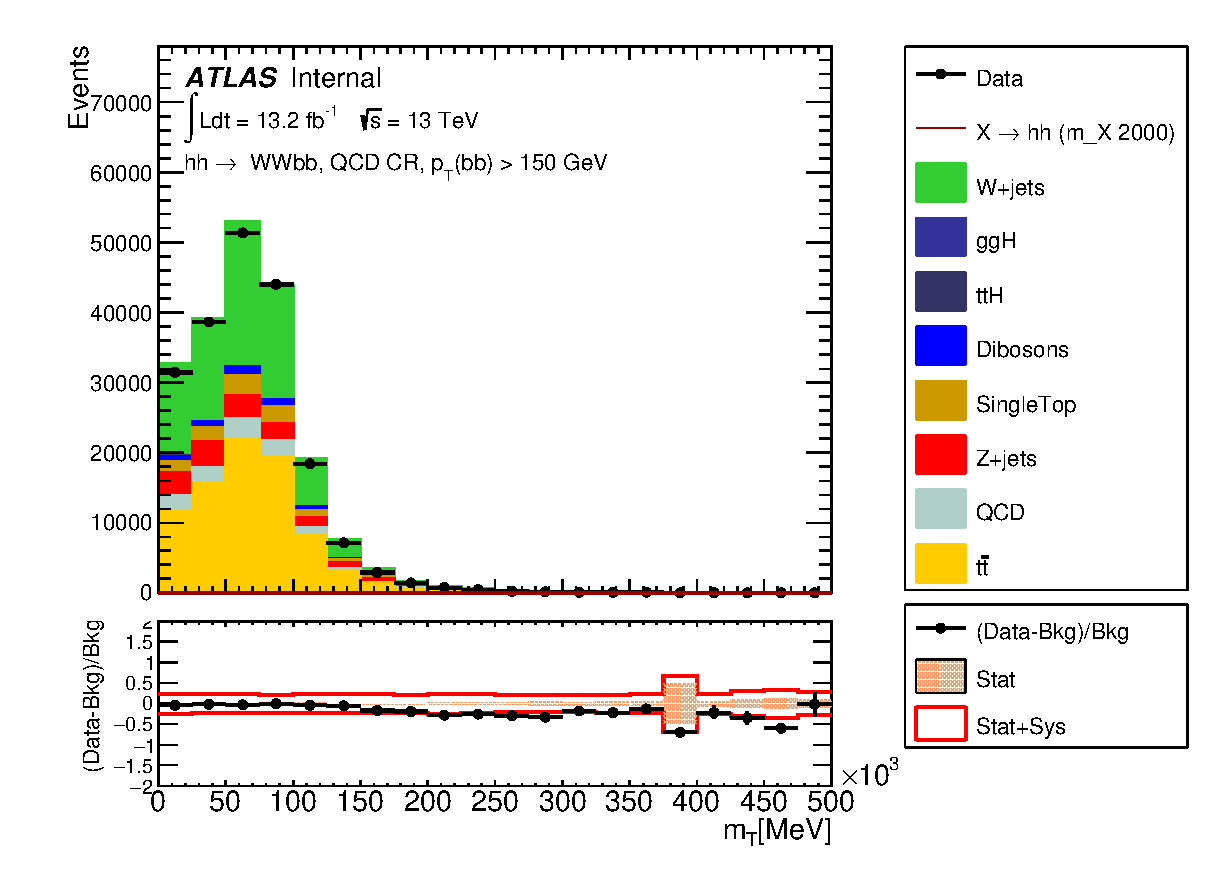
\includegraphics[width=0.47\textwidth, height=0.35\textwidth]{chapters/dihiggs/figures/C_bj1_opt700_bbpt150_wlepmtben.eps}
\includegraphics[width=0.47\textwidth, height=0.35\textwidth]{chapters/dihiggs/figures/ControlPlots/CR1/C_opt700_bbpt150_wlepmtben.eps}
\end{center}
\caption{$m_{\rm T}$ distribution for events in the QCD enriched control region
   with one $b$-tag (left) and with $t\bar{t}$ control region two $b$-tag (right).}
\label{fig:mwt}
\end{figure}







